\chapter{Дартмудский диалог} 

«Холодная война» прочно ассоциируется с такими интересными вещами, как взаимное недоверие, паранойя и демонизация. Действительно, по большей части так и было — политики бросались громкими обвинениями, дипломаты сверлили друг друга стальными взглядами, военные упражнялись во взаимном устрашении, а народ активно делился стереотипами и страхами на прокуренных кухнях. Однако есть и пример, когда обе стороны попытались преодолеть стену непонимания, собрав своих влиятельных общественных деятелей за стол переговоров. Речь пойдет о «Дартмутском диалоге» — неправительственной конференции, ставшей светочем здравого смысла во время Карибского кризиса.

К концу 50-х годов XX века в правящих кругах обеих сверхдержав начинают догадываться, что дипломатия как-то не задается. Ещё на XX съезде КПСС Микоян сетовал на то, как «страна серьезно отстает в анализе как капиталистического, так и некапиталистического развития». В 1959-м похожую мысль излагает и Эйзенхауэр, говоря о необходимости диалога с другими народами. По сути, обе стороны признались в непонимании друг друга — из-за взаимных предрассудков нормальный диалог не клеился. Необходимо было найти новый путь к компромиссу и взаимопониманию.

Решение предложил Норман Казинс — редактор крупного американского журнала Saturday Review, и сооснователь организации по ядерному разоружению SANE. Выступая в июне 1959 г. перед президиумом Советского комитета защиты мира, он предложил собрать представителей двух стран для совместного обсуждения насущных проблем — и там же получил одобрение с советской стороны. Чуть позже свое согласие дал и Эйзенхауэр, и уже в ноябре 1960 г. в студенческом городке Дартмутского колледжа проходит первая конференция (хотя последующие конференции будут проходить в совершенно других городах, название «Дартмутская» останется).
\begin{figure}[h!tb] 
	\centering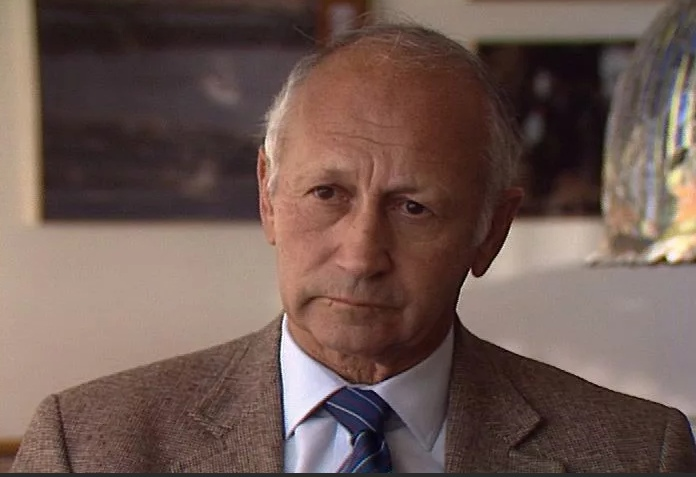
\includegraphics[scale=0.5]{Dartmud/pqA6Euw_ISE.jpg}
	%	\label{fig:scipion} % Unique label used for referencing the figure in-text\end{document}
	%	%\addcontentsline{toc}{figure}{Figure \ref{fig:placeholder}} % Uncomment to add the figure to the table of contents%----------------------------------------------------------------------------------------
	\caption{Норман Казинс (1915 - 1990). Очень интересный персонаж, ярый противник ядерного оружия, "человек, рассмешивший смерть". Явно достоин отдельной заметки, а то и статьи. }%	CHAPTER 2
\end{figure}
Первая делегация состояла из людей, приближенных к политическим кругам СССР и США. Советскую делегацию возглавлял писатель А. Корнейчук, близкий друг Хрущева и член Верховного Совета СССР и Украины. Помимо него в делегации были: экономист Модест Рубинштейн, композитор Вано Мурадели, писатель Борис Полевой, ученый-правовед Виктор Чхиквадзе, режиссер Сергей Юткевич. С американской стороны, помимо Казинса, в конференции участвовали: бизнесмен Уильям Бентон, дипломат Джордж Фрост Кеннан, юрист Ричард Легхарн. Список участников неполный, но суть вы уловили: обе делегации были разношерстными по родам деятельности и интересам. Например, Кеннан, в прошлом сотрудник посольства в Москве, был известен концепцией «сдерживания коммунизма», а самого Казинса в СССР считали ярым антисоветчиком и достаточно долго относились к нему с недоверием.

На первых трех встречах обсуждали контроль вооружений, роль СССР и США в развитии стран «третьего мира», научный и культурный обмен между странами, участие граждан во внешней политике и прочее. Больше всего споров вызвало обсуждение разоружения, особенно на фоне проходившего примерно в то же время Женевского процесса, где куча экспертов тщетно пытались добиться компромисса в вопросе запрета ядерных испытаний. Проблема была в том, что советская сторона упорно не соглашалась на разрешение инспекций подземных ядерных взрывов, аргументируя это тем, что современная на тот момент техника уже позволяла фиксировать взрывы. Фактически же Союз опасался, что инспекции будут лишь прикрытием для шпионажа. Делегаты Дартмутских встреч были чуть успешнее женевских, т.к. смогли понять эту причину и предложить компромисс: вводить инспекции не сразу, а постепенно, чтобы у обеих стран не было сомнений в честности проверок. Казалось бы, достаточно простой выход, зачем для этого нужны какие-то там неофициальные встречи? Но именно благодаря такому формату, делегатам удалось наладить доверительные отношения и выстроить объективный диалог, без заученных пропагандистских лозунгов и сухого официоза.
\begin{figure}[h!tb] 
	\centering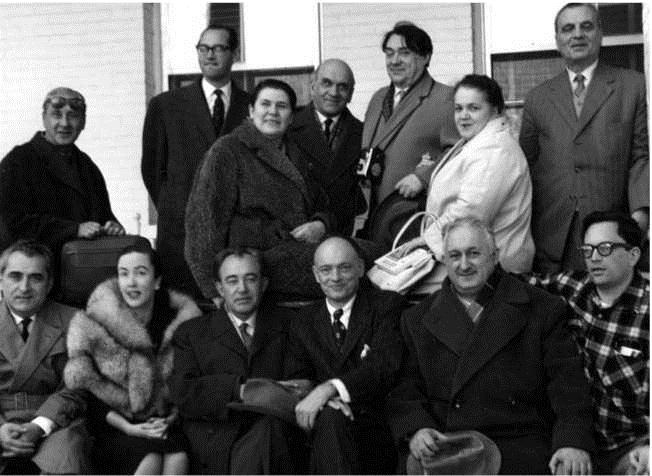
\includegraphics[scale=0.5]{Dartmud/-6ky6zoSgDI.jpg}
	%	\label{fig:scipion} % Unique label used for referencing the figure in-text\end{document}
	%	%\addcontentsline{toc}{figure}{Figure \ref{fig:placeholder}} % Uncomment to add the figure to the table of contents%----------------------------------------------------------------------------------------
	\caption{Президент Дартмутского Колледжа Джон Дики вместе с советской делегацией. Хановер, Нью-Гэмпшир, 1960 }%	CHAPTER 2
\end{figure}
Звездный час для Дартмутского диалога наступил во время Карибского кризиса, на Третьей Дартмутской конференции в городе Андовере, штат Массачусеттс, проходившей с 21 по 27 октября 1962 года. День открытия прошел довольно спокойно, а вот на следующий день президент Кеннеди объявил всему миру о советских ракетах на Кубе, и обстановка резко накалилась. Стороны, однако, не отказались от диалога, и конференция продолжилась — участники принялись искать выход из кризиса. Собственно, ровно через день крепко связанная с Казинсом SANE направит в администрацию США предложение демонтировать американские ракеты в Турции в обмен на демонтаж советских ракет на Кубе — и в этот же день то же самое предложение Роберт Кеннеди озвучит в разговоре с посредником Москвы Георгием Большаковым (о его роли в советско-американских отношениях я писал в прошлый раз). Конечно, нельзя исключать, что братья Кеннеди пришли к этому варианту задолго до Дартмутской встречи — в конце концов, у американцев была фора длиною в неделю после подтверждения наличия ракет на Кубе, и наверняка Белый дом хорошо подготовился к давлению на Советский Союз. В любом случае, предложение Кеннеди поступит в Москву лишь 25 октября, а пока что у Хрущева еще имеется свой план.

Советская сторона Дартмутской встречи предлагала и другой вариант решения кризиса — личную встречу Хрущева и Кеннеди. Что характерно, примерно в то же время Хрущев через бизнесмена У. Э. Нокса передал в Вашингтон сообщение примерно того же толка. Сходство не случайно — среди делегатов были люди, находившиеся в прямом контакте с Москвой на протяжении всей конференции. Впрочем, американская сторона отвергла предложение. Их собственный вариант, подразумевавший десятидневный мораторий на перехват советских судов и создание специальной комиссии ООН по выходу из кризиса, был также отвергнут. Компромисс пришел откуда не ждали — из Ватикана. Отец Феликс Морлион, представитель Ватикана, формально не участвовал в сугубо двустороннем диалоге, но Казинс по-дружески позволил ему выступить с заявлением. Говоря от имени Папы Римского, Морлион призвал мировых лидеров к моральной ответственности и предложил советам отозвать все суда с Кубы, а Штатам — прекратить блокаду острова. Обе делегации донесли это предложение до своих правительств. Что удивительно: советская сторона, в целом, с предложением согласилась; Хрущев заявил, что полностью поддерживает предложение Папы. А вот Кеннеди предложение отверг.
\begin{figure}[h!tb] 
	\centering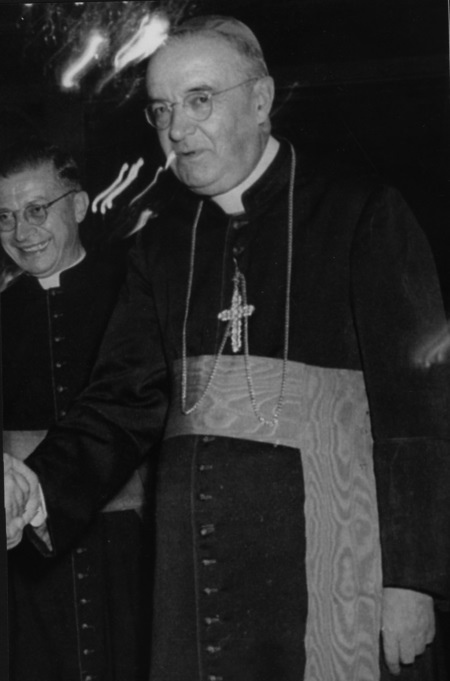
\includegraphics[scale=0.5]{Dartmud/yUSfxNuIlFI.jpg}
	%	\label{fig:scipion} % Unique label used for referencing the figure in-text\end{document}
	%	%\addcontentsline{toc}{figure}{Figure \ref{fig:placeholder}} % Uncomment to add the figure to the table of contents%----------------------------------------------------------------------------------------
	\caption{Если искать в интернете инфу про отца Морлиона, то найдется очень много различной литературы про знаменитых шпионов. Так или иначе, за Морлионом закрепилось звание агента ЦРУ — что, судя по найденной мною инфе, неудивительно. Я не очень в шпионских делах - может, когда-нибудь... }%	CHAPTER 2
\end{figure}
Собственно, роль Дартмутского диалога в разрешении кризиса на этом заканчивается — загнанное в угол советское правительство, отчаянно пытавшееся на ходу продумать стратегию поведения, ухватилось за предложение обмена ракетами, и в итоге ключевую роль в разрешении кризиса сыграет прямая переписка между Кеннеди и Хрущевым. Стоит, впрочем, упомянуть, что в ходе конференции отец Морлион обратится к советской делегации с просьбой назначить Казинса неофициальным посредником Ватикана, дабы восстановить разорванные отношения с Москвой. Советское правительство, впечатленное ролью Морлиона в урегулировании кризиса, даст добро, и уже в декабре Казинс, предварительно встретившись с президентом Кеннеди, отправится в Москву на встречу лично с Хрущевым. Будучи формально представителем Ватикана, Казинс будет обсуждать с Хрущевым вопросы отношений США и СССР. Забегая вперед, скажу, что Казинс сыграет важную роль в заключении договора об ограничении ядерных испытаний 1963 года — договора, заключенного, во многом, на советских условиях. Таким образом, благодаря Дартмуту-3 советско-американская неофициальная дипломатия получила нового посредника взамен раскрытого Большакова, а Советский Союз впоследствии достиг дипломатического успеха.

Всего Дартмутских встреч до развала СССР было 17 – последняя прошла в Ленинграде, в июле 1990 года. В последние годы в рамках конференции были созданы целевые группы решения различных вопросов (Specialized Task Forces). Эти группы создавались для решения конкретных вопросов, и, в отличие от Дартмутских встреч, пережили распад СССР и продолжают созываться до сих пор. А сами Дартмутские встречи были возрождены в 2014 году, на фоне обострения отношений между Россией и США. К 2016 году было проведено 5 Дартмутских встреч (что характерно, ни одна из конференций, кроме самой первой, в Дартмуте более не проводилась), и на них обсуждались известные нам вопросы Украины, Сирии, отношений РФ и НАТО, и прочие. Последние новости с упоминанием Дартмутского диалога довольно свежие — в прошлом году обеспокоенные участники просили власти РФ и США продлить СНВ-3, а в этом медицинская целевая группа обсуждала опасность COVID-19. Об эффективности современного Дартмута, как говорится, делайте выводы сами.

А Дартмут эпохи Холодной войны так и останется смелым примером того, как неформальные контакты могут помочь в ситуации, когда не справляется дипломатия официальная.

P. S. По запросу «Дартмутский диалог» в Гугле можно также найти информацию о Дартмутском семинаре. Это мероприятие, проведенное в 1956 году, было посвящено вопросу искусственного интеллекта, и никак не связано с Дартмутским диалогом. Не путайте!

Автор Алексей Иванов.  Оригинал \url{https://vk.com/wall-162479647_237732}

\#Иванов@catx2
\#Заметка@catx2




